\documentclass[8pt]{beamer}

\mode<presentation>
{
  \usetheme{AnnArbor}
  \usecolortheme{beaver}
  \usefonttheme{default}
  \setbeamertemplate{caption}[numbered]
  \setbeamercovered{transparent}
  \usefonttheme[onlymath]{serif}
  \setbeamertemplate{itemize items}[default]
  \setbeamertemplate{navigation symbols}{\insertslidenavigationsymbol\insertframenavigationsymbol}
}
\usepackage[english]{babel}
\usepackage[utf8x]{inputenc}
\usepackage{mathtools, xcolor, soul, amsfonts, appendixnumberbeamer, graphicx, tikz, subcaption, commath}
\usepackage[makeroom]{cancel}
\usepackage[justification=centering]{caption}
\usepackage{graphicx}
\usepackage[export]{adjustbox}
\graphicspath{ {images/} }
%\hypersetup{pdfpagemode=FullScreen}

\title[\scalebox{.8}{Obstacle Avoidance 101}]{Obstacle Avoidance 101}
\author[\scalebox{.8}{Dariush Hasanpoor}]{Dariush Hasanpoor}
\institute[]{Isfahan University Of Technology}
\date[\scalebox{.8}{Isfahan University Of Technology}]{Feb. 2016}

\newcommand{\Xtri}{$\blacktriangleright$ }
\newcommand{\Ytri}{$\triangleright$ }
\newcommand{\itemXtri}{\item[\Xtri]}
\newcommand{\itemYtri}{\item[\Ytri]}
\renewcommand{\|}[1][.3em]{\hspace{#1}|\hspace{#1}}
\renewcommand{\,}[1][.3em]{,\hspace{#1}}
\newcommand\Wider[2][3em]{%
\makebox[\linewidth][c]{\begin{minipage}{\dimexpr\textwidth+#1\relax}\raggedright#2\end{minipage}}}
\newcommand*{\Scale}[2][4]{\scalebox{#1}{$#2$}}%

\definecolor{light-blue}{HTML}{66AFE9}
\definecolor{light-red}{HTML}{F77B7B}
\definecolor{light-green}{HTML}{87D13E}

\newcommand{\subitem}[1]{{\setlength\itemindent{12pt}\item[\Ytri] #1}}
\newcommand{\subsubitem}[1]{{\setlength\itemindent{24pt}\item[$\bullet$] #1}}
\newcommand{\morespace}{\setlength\itemsep{1em}}

\makeatletter
% The following two commands should only be given between frames

% Remove the equation counter from the list of counters that are reset after
% each overlay.
\def\donotresetequations{{%
    \let\@@elt\relax
    \def\@elt##1{%
        \expandafter\ifx\csname ##1\endcsname\c@equation%
        \else%
            \@@elt {##1}%
        \fi%
    }%
    \edef\beamer@overlaycounterresets{\beamer@overlaycounterresets}%
    \let\@elt\relax%
    \def\@@elt{\@elt}%
    \xdef\beamer@overlaycounterresets{\beamer@overlaycounterresets}%
}}

% Add the equation counter from the list of counters that are reset after
% each overlay.
\def\resetequations{\resetcounteronoverlays{equation}}
\makeatother

\donotresetequations

\begin{document}

\begin{frame}
  \titlepage
\end{frame}

\begin{frame}{Outline}
  \tableofcontents[hideallsubsections]
\end{frame}

\section{Introduction}
\frame{\tableofcontents[currentsection]}

\begin{frame}{What is a Obstacle Avoidance?}
\begin{block}{According to Wikipedia:}
In robotics, obstacle avoidance is the task of satisfying some control objective subject to non-intersection or non-collision position constraints.
\end{block}
\end{frame}

\section{Obstacle Avoidance Algorithms}
\frame{\tableofcontents[currentsection]}
\subsection{Bug Algorithms}
\frame{\tableofcontents[currentsubsection]}
\begin{frame}{The Bugs!}
\begin{itemize}
\morespace
\only<1>{
\item Many planning algorithms assume global knowledge.
\item Bug algorithms assume only local knowledge of the environment and a global goal.
\item The Bug algorithms\cite{lumelsky1990incorporating, lumelsky1990path}, are simple ways to overcome unexpected obstacles in the robot motion from a start point $s$, to a goal point $g$.
\item The goal of the algorithms is to generate a collision free path from the $s$ to $g$ with the underlying principle based on \emph{contouring the detected obstacles}.
\item Bug 1 and Bug 2 assume essentially tactile sensing.
}
\only<2>{
\item The general procedure in bugs:
    \subitem Move towards the goal, unless an obstacle is encountered.
    \subitem Circumnavigate the obstacle until motion toward the goal is again allowable.
\item Robot is assumed to be a point with perfect positioning.
\item Robot has a contact sensor which detects the obstacle boundary if it touches it.
\item The robot can measure the distance $d(x,y)$ between any two points.
\item The workspace is bounded.}
\end{itemize}
\end{frame}
\begin{frame}{Bug 1}
\begin{itemize}
\morespace
%\only<1>{
%\item Bug1 exhibits two behaviors:
%    \subitem{motion to goal.}
%    \subitem{boundary following.}
%\item The robot moves along a line from $s$ to $g$.
%\item As soon as an obstacle $i$ is detected, the robot does a full contour around it, starting at the hit point $H_i$.
%\item The full contour aims at evaluating the point of minimum distance to the target, $L_i$ which is named as the leave point.
%\item The robot then continues the contouring motion until reaching the $L_i$ point again, from where it leaves along a straight path to the target.}
\only<1>{
\item[] \begin{figure}
\centering
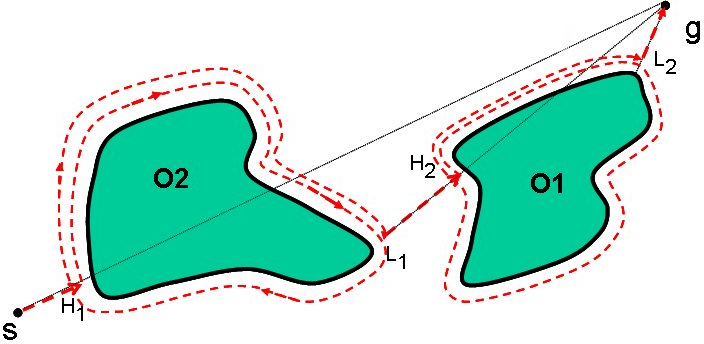
\includegraphics[scale=1]{bug1}
\caption{Representing a situation in bug1 with two obstacles where $H_1$ and $H_2$ are the hit points and $L_1$ and $L_2$ the leave points.}
\end{figure}
}
\end{itemize}
\end{frame}
\begin{frame}{Bug 2}
\begin{itemize}
\morespace
%\only<1>{
%\item In the Bug2 algorithm the obstacle contour starts at the hit point $H_i$ but ends whenever the robot crosses the line to the target.
%\item This defines the leave point $L_i$ of the obstacle boundary-following behavior.
%\item From $L_i$ the robot moves directly to the target.
%\item The procedure repeats if more obstacles are detected.}
\only<1>{
\item[] \begin{figure}
\centering
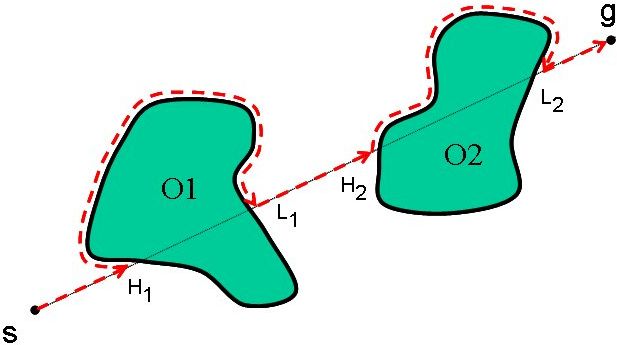
\includegraphics[scale=1]{bug2}
\caption{Representing a situation in bug2 with two obstacles where $H_1$ and $H_2$ are the hit points and $L_1$ and $L_2$ the leave points.}
\end{figure}
}
\end{itemize}
\end{frame}
\begin{frame}{Pros and Cons}{Bug1 vs. Bug2}
\begin{itemize}
\morespace
\only<1>{\item[] \begin{figure}
    \centering
    \begin{subfigure}{0.4\textwidth}
    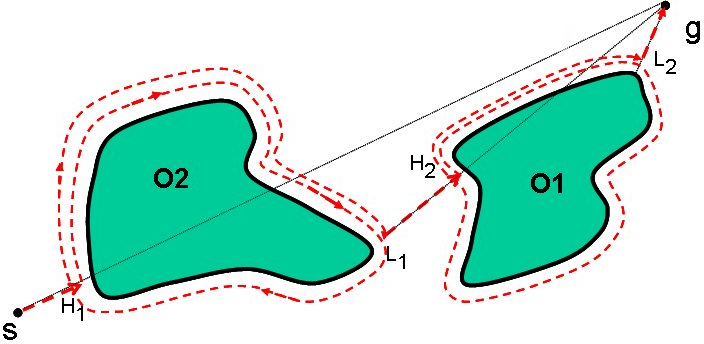
\includegraphics[width=\textwidth]{bug1}
    \caption{The bug1 behaviour}
    \end{subfigure}
    \begin{subfigure}{0.4\textwidth}
    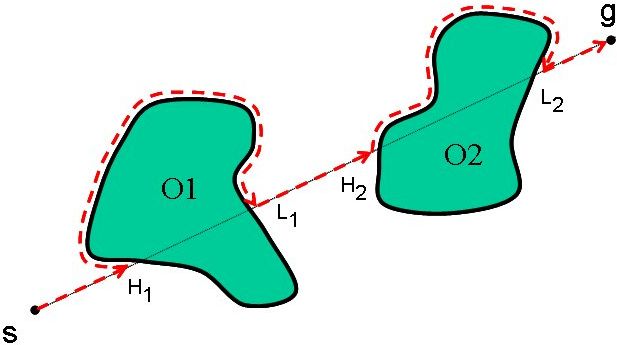
\includegraphics[width=\textwidth]{bug2}
    \caption{The bug2 behaviour}
    \end{subfigure}
    \caption{The difference between different version of bug algorithm}
\end{figure}}
\only<2>{\item Bug1:
    \subitem{Is an exhaustive search algorithm; it looks at all choices before commiting. therefor it's very inefficient but guarantees that the robot will reach any reachable goal.}
\item Bug2: 
    \subitem{Is a greedy algorithm; it takes the first thing that looks better.}
\item In many cases, bug2 has a shorter travel time than Bug 1 algorithm and is more efficient specially in open spaces.
    \subitem{The bug1 has a more predictable performance overall.}}
\only<3>{
\item None of these algorithms take robot kinematics into account which is a severe limitation, specially in the case of \emph{non-holonomic} robots.
    \subitem{A robot is \emph{holonomic} if all the constraints that it is subjected to are integrable into positional constraints.}}
\end{itemize}
\end{frame}
%\begin{frame}{Tangent Bug}
%\end{frame}

\subsection{The Potential Field Methods}
\frame{\tableofcontents[currentsubsection]}
\begin{frame}{The Potential Field Methods}
\only<1>{\begin{itemize}
\morespace
\item The robot is consider as a particle that moves immersed in a potential field generated by the goal and by the obstacles present in the environment\cite{khatib1986real}.
\item The goal generates an attractive potential while each obstacle generates a repulsive potential.
\item The robot immersed in the potential filed is subject to the action of a force that drives it to the goal.
\end{itemize}}
\only<2>{
\begin{block}{A point of view in PF}
\begin{itemize}
\morespace
\item A potential field can be viewed as an energy field and so its gradient, at each point, is a force.
\item In this analogy, the robot is a positive charge, the goal is a negative charge and the obstacles are sets of positive charges.
\end{itemize}
\end{block}}
\begin{itemize}
\morespace
\item[]
\only<3>{\item Let $q$ represent the position of the robot, considered as a particle moving in a n-dimensional space $R^n$.
\item The artificial potential field where the robot moves is a scalar function $U(q):R^n\rightarrow R$:
\begin{align}
U(q) &= U_{\text{att}}(q) + U_{\text{rep}}(q)\nonumber\\
&= U_{\text{att}}(q) + \sum_i U_{\text{rep}_i}(q)
\end{align}}
\only<4>{
\item{The attractive potential is chosen to be zero at the goal and to increase as the robot is far away from the goal.}
\item{The repulsive potential, associated with each obstacle, is very high (infinity) in the close vicinity of the obstacles and decreases when
the distance to the obstacle increases.}}
\only<5>{
\item The force that drives the robot is the negative gradient of the artificial potential, i.e.
\begin{equation}
F(q) = F_{\text{att}}(q) + F_{\text{rep}}(q) = - \nabla U_{\text{att}}(q) - \nabla U_{\text{rep}}(q)\label{eq:force_nabla_U}
\end{equation}
    \subitem{This force can be considered as the velocity vector that drives the point robot.}
}
\end{itemize}
\end{frame}
\begin{frame}{The Potential Field Methods}{The Attractive Potential}
\begin{itemize}
\morespace
\only<1>{\item The usual choice for the attractive potential is the standard parabolic that grows quadratically with the distance to the goal:
\begin{equation}
U_{\text{att}}(q) = {1 \over 2}k_{\text{att}}d^2_{\text{goal}}(q)
\end{equation}
    \subitem{Where $d_{\text{goal}}(q) = \norm{q-q_{\text{goal}}}$ is the Euclidean distance of the robot (considered at $q$), to the goal, at $q_{\text{goal}}$ and $k_{\text{att}}$ is a scaling factor.}
\begin{align}
\nabla U_{\text{att}} &= k_{\text{att}}(q-q_{\text{goal}})\\
F_{\text{att}} &= -\nabla U_{\text{att}} = -k_{\text{att}}(q-q_{\text{goal}})
\end{align}
}
\only<2>{
\item[] \begin{figure}
    \centering
    \begin{subfigure}{0.4\textwidth}
    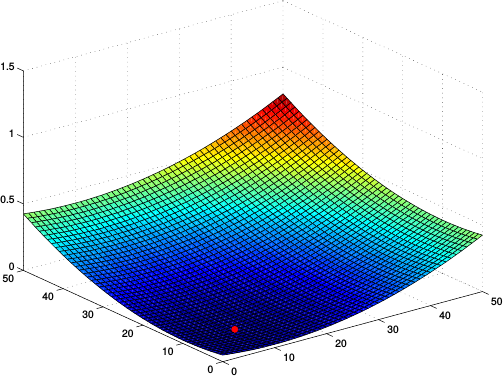
\includegraphics[width=\textwidth]{pf_1}
    \caption{Attractive Potential}
    \end{subfigure}
    \begin{subfigure}{0.4\textwidth}
    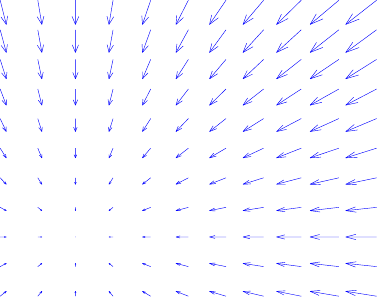
\includegraphics[width=.93\textwidth]{pf_2}
    \caption{Attractive Force to the goal}
    \end{subfigure}
    \caption{The Potential Field Methods -- the goal at (10, 10) is represented by a mark.}
\end{figure}}
\end{itemize}
\end{frame}
\begin{frame}{The Repulsive Potential}
\begin{itemize}
\morespace
\only<1>{
\item The repulsive potential keeps the robot away from the obstacles.
\item The repulsive potential is stronger when the robot is closer to the obstacle and has a decreasing influence when the robot is far away.
\item Given the linear nature of the problem:
\begin{gather}
U_{\text{rep}} = \sum_i U_{\text{rep}_i}(q)\\
U_{\text{rep}_i} = \begin{cases}
{1 \over 2}k_{\text{obst}_i}\Bigg({1 \over d_{\text{obst}_i}(q)}-{1 \over d_0}\Bigg)^2 & \text{if } d_{\text{obst}_i}(q) < d_0\\
0 & \text{o.w.}
\end{cases} 
\end{gather}
where:
    \subitem{$d_{\text{obst}_i}(q)$ is the minimal distance from $q$ to the obstacle $i$.}
    \subitem{$k_{\text{obst}_i}$ is a scaling constant.}
    \subitem{$d_0$ is the obstacle influence threshold.}}
\only<2>{
\item The negative of the gradient of the repulsive potential, $F_{\text{rep}_i}(q) = -\nabla U_{\text{rep}_i}(q)$, is given by,
\begin{equation}
F_{\text{rep}_i} = \begin{cases}
k_{\text{obst}_i}\Bigg({1 \over d_{\text{obst}_i}(q)}-{1 \over d_0}\Bigg) \cdot {q - q_{\text{obst}_i} \over d^3_{\text{obst}_i}(q)} & \text{if } d_{\text{obst}_i}(q) < d_0\\
0 & \text{o.w.}
\end{cases} 
\end{equation}
\begin{figure}
    \centering
    \begin{subfigure}{0.4\textwidth}
    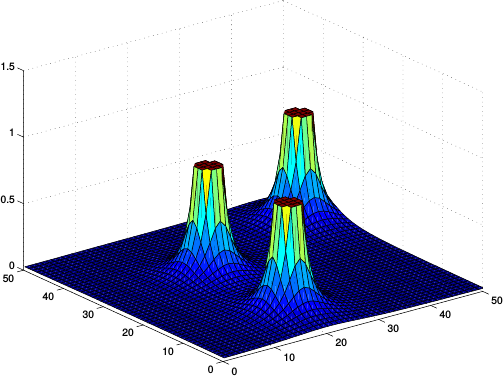
\includegraphics[width=\textwidth]{pf_3}
    \caption{Repulsive Potential}
    \end{subfigure}
    \begin{subfigure}{0.4\textwidth}
    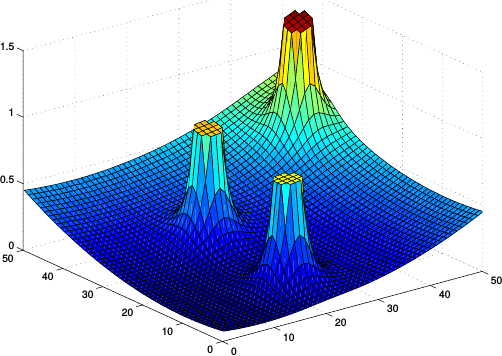
\includegraphics[width=\textwidth]{pf_4}
    \caption{Attractive+Respulsive Potential}
    \end{subfigure}
    \caption{The Potential Field Methods}
\end{figure}}
\end{itemize}
\end{frame}
\begin{frame}{The Potential Field Methods}{Pros and Cons}
\begin{itemize}
\morespace
\item The potential field approach herein presented is a simple path planning.
\item For a static and completely known environment, the potential can be evaluated off-line providing the velocity profile to be applied to a point robot moving in the energy field from a starting point to a goal.
\item Also, the technique can be applied in an on-line version that accommodates an obstacle avoidance component.
\item The robot using this approach can stuck in a local minimum:
\begin{figure}
\centering
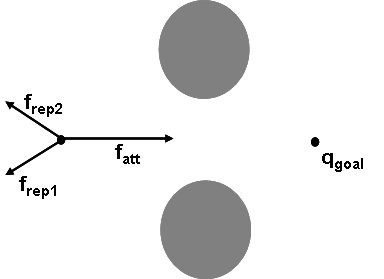
\includegraphics[scale=1]{pf_local_min}
\caption{Local minimum of the total potential due to environment symmetry}
\end{figure}
\end{itemize}
\end{frame}
\begin{frame}{The Potential Field Methods}{Other Versions}
\begin{itemize}
\morespace
\item In some extended version of the potential field based methods, the repulsive potential is changed in some ways\cite{khatib1986real,khatib1995extended}.
\subitem{The repulsive force due to an obstacle is not only considered as a function of the distance to the obstacle but also of the orientation of the robot relative to the obstacle. This is a reasonable change since the urgency of avoiding an obstacle parallel to the robot motion is clearly less than the one that arises when the robot moves directly facing the obstacle.}
\subitem{The second extension of the repulsive potential does not consider the obstacles that will not closely affect the robot velocity. For example, it is irrelevant to consider the repulsive force generated by an obstacle in the back of the robot, when it is moving forward.}
\end{itemize}
\end{frame}
\subsection{The Virtual Force Field}
\frame{\tableofcontents[currentsubsection]}
\begin{frame}{The Virtual Force Field}
\begin{itemize}
\morespace
\only<1>{\item The Virtual Force Field(VFF) method is one of earlier real-time obstacle avoidance method for fast-running vehicles\cite{borenstein1989real}.
\item Advantage of using VFF instead of previous methods:
    \subitem{It's fast.}
    \subitem{It's continuous.}
    \subitem{Smooth motion of the controlled vehicle among unexpected obstacles.}
    \subitem{Does not require the vehicle to stop in front of obstacles.}}
\only<2>{
\item The individual components of the VFF method are presented below.
    \subitem{The VFF method uses a two-dimensional Cartesian histogram grid $C$ for obstacle representation.}
        \subsubitem{Each cell $(i,j)$ in the histogram grid holds a certainty value, $c_{i,j}$.}
        \subsubitem{The histogram grid differs from the certainty grid in the way it is built and updated}
    \subitem{Using the grid's value the VFF applies the PF idea to the histogram grid, so the probabilistic sensor information can be used efficiently to control the vehicle.}}
\only<3>{
\item[] \begin{figure}
\centering
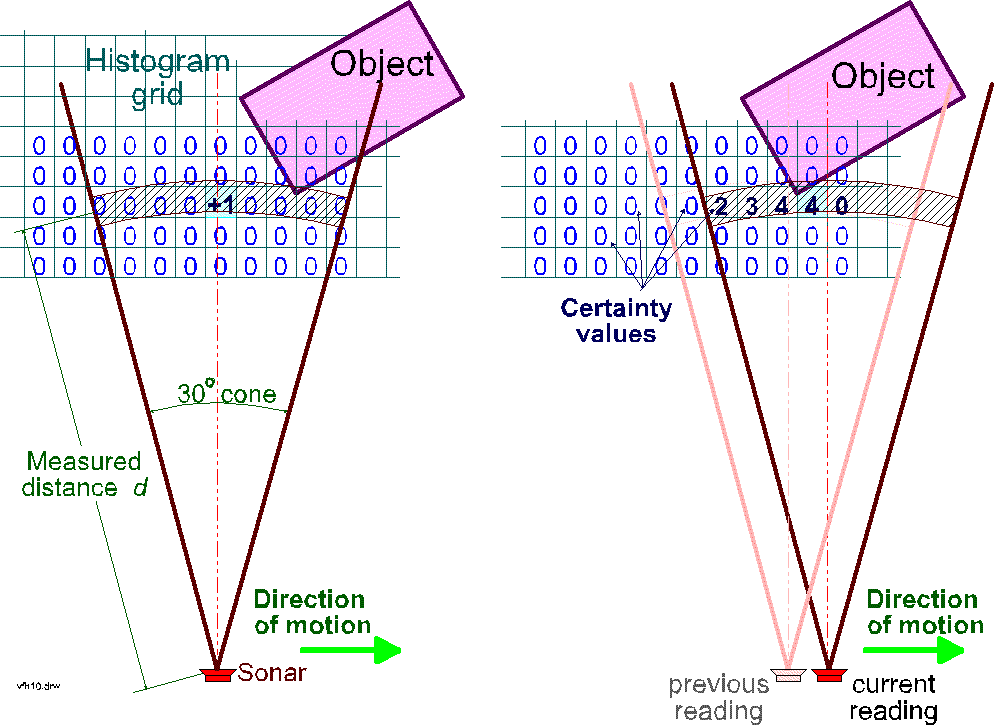
\includegraphics[width=.7\textwidth]{vff_grid}
\caption{Construction of the 2D Histogram grid map.}
\end{figure}
}
\only<4>{
\item[] \begin{figure}
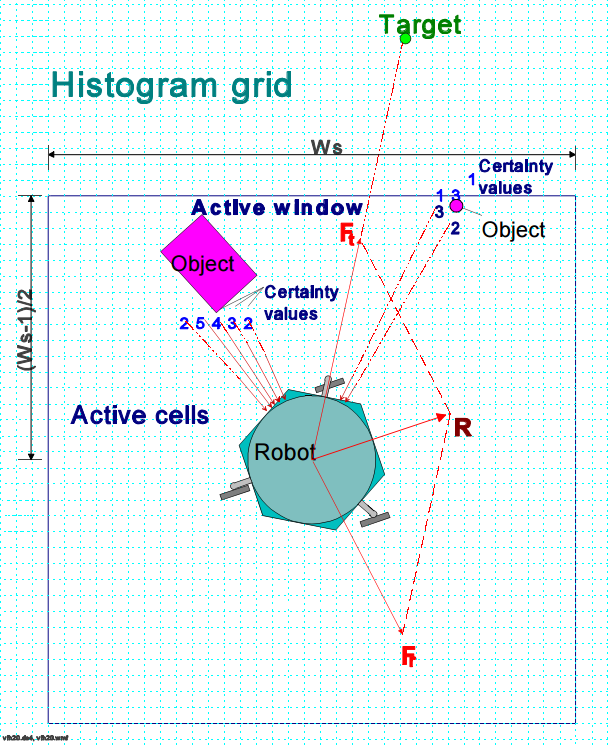
\includegraphics[width=.5\textwidth]{vff_active_window}
\end{figure}
}
\only<5>{
\item As the robot moves around, range readings are taken and projected into the Certainty Grid, as explained.
\item Simultaneously, the algorithm scans a small square window of the grid.
\item The size of the window is $33\times 33$ cells(i.e., $3.30\time 3.30$m) and its location is such that the robot is always at its center.
\item Each occupied cell inside the window applies a repulsive force to the robot, "pushing" the robot away from the cell.
}
\only<6>{
\item  The magnitude of this force is proportional to the cell contents, $C(i,j)$, and is inversely proportional to the square of the distance between the cell and the robot:
\begin{equation}
F(i,j) = {F_{cr}C(i,j) \over d^2(i,j)}\Bigg[{x_t - x_0 \over d(i,j)}\hat{x} + {y_t - y_0 \over d(i,j)}\hat{y}\Bigg] 
\end{equation}
\item where:
    \subitem{$F_{cr}$ Force constant (repelling)}
    \subitem{$d(i,j)$ Distance between cell $(i,j)$ and the robot}
    \subitem{Certainty level of cell $(i,j)$}
    \subitem{Robot's present coordinates}
    \subitem{Coordinates of cell $(i,j)$}
\item The resultant repulsive force, $F_r$, is the vectorial sum of the individual forces from all cells: \[F_r = \sum_{i,j} F(i,j)\]
}
\only<7>{
\item At any time during the motion, a constant-magnitude attracting force, $F_t$, pulls the robot toward the target.
\item $F_t$ is generated by the target point $t$, whose coordinates are known to the robot. The target-attracting force $F_t$ is given by:
\begin{equation}
F_t = F_{cr}\Bigg[{x_t - x_0 \over d(t)}\hat{x} + {y_t - y_0 \over d(t)}\hat{y}\Bigg] 
\end{equation}
\item The vectorial sum of all forces, repulsive from occupied cells and attractive from the target position, produces a resultant force vector $R$:
\begin{equation}
R = F_t + F_r
\end{equation}
}
\end{itemize}
\end{frame}
\begin{frame}{The Virtual Force Field}{Pros and Cons}
\begin{itemize}
\morespace
\item Some of VFF limitation and disadvantages are\cite{borenstein1991vector}:
    \subitem Force-based obstacle-avoidance methods do not allow the robot to pass through narrow passages.
    \subitem Instability of motion when traveling within narrow corridors.
\item So \emph{The Vector Field Histogram}(VFH) was introduced to improve the VFF method.
    \subitem VFH control results in smooth motion of the controlled vehicle among densely cluttered and unexpected obstacles.
    \subitem A VFH controlled vehicle can easily enter narrow passages and can travel in narrow corridors at high speeds and without oscillations.
\end{itemize}
\end{frame}
\subsection{The Vector Field Histogram}
\frame{\tableofcontents[currentsubsection]}
\begin{frame}{The Vector Field Histogram}
\begin{itemize}
\morespace
\only<1>{
\item The VFH method uses a two-dimensional Cartesian Histogram Grid for the representation of obstacles(like VFF method)\cite{borenstein1991vector}.
\item The VFH method employs a two-stage data reduction technique, in which three levels of data representation can be distinguished.
    \subitem level 1) The highest level holds the detailed description of the robot's environment.
    \subitem level 2) At the intermediate level, a Polar Histogram $H$ is constructed around the robot's momentary center.
    \subitem level 3) The lowest level of data representation is the output of the VFH algorithm.
}
%\only<2>{
%\item Level 1) The highest level holds the detailed description of the robot's environment:
%    \subitem In this level, the two-dimensional Cartesian Histogram Grid C is continuously updated in real-time with range data sampled by the onboard range sensors.
%    \subitem The Histogram Grid is absolute and does not change with the robot's momentary location.
%}
\only<2>{
\item Level 2) At the intermediate level, a Polar Histogram $H$ is constructed around the robot's momentary center:
    \subitem{$H$ comprises $n$ angular sectors of width $\alpha$}
        \subsubitem{$\alpha$ may be chosen arbitrarily but must be such that $n={360\over \alpha} \in \mathbb{N}^+$}
    \subitem A transformation maps $C^*$ into $H$ resulting in each sector $k$ holding a value $h_k$ which represents the polar obstacle density in the direction $k$.
}
\only<3>{
\item Level 3) The lowest level of data representation is the output of the VFH algorithm:
    \subitem The reference values for the drive and steer controllers of the vehicle.
}
\end{itemize}
\end{frame}
\begin{frame}{The Vector Field Histogram}{Stage 1/2 of data reduction}
\begin{columns}
\begin{column}{0.5\textwidth}
\begin{itemize}
\item[] \begin{gather}
\beta_{i,j} = tg^{-1}\Big({y_j - y_0 \over x_j - x_0}\Big)\\
m_{i,j} = (C^*)^2(a-bd_{i,j}) 
\end{gather}
\item Where:{\footnotesize
    \subitem{$a,b$ Positive constants.}
    \subitem{$d_{i,j}$ Distance between active cell $(i,j)$ and the VCP.}
    \subitem{$c^*_{i,j}$ Certainty value of active cell $(i,j)$.}
    \subitem{$m_{i,j}$ Magnitude of the obstacle vector at cell $(i,j)$.}
    \subitem{$x_0, y_0$ Present coordinates of the VCP.}
    \subitem{$x_i, y_j$ Coordinates of active cell $(i,j)$.}
    \subitem{$\beta_{i,j}$ Direction from active cell $(i,j)$ to the VCP.}
\item $a,b$ are choosen such that $a - bd_{\max} = 0$ where $d_{\max} = \sqrt{2}(w_s - 1)/2$ is the distance between the farthest \emph{active cell} and the VCP.}
\end{itemize}
\end{column}
\begin{column}{0.5\textwidth}
    \begin{figure}\centering
        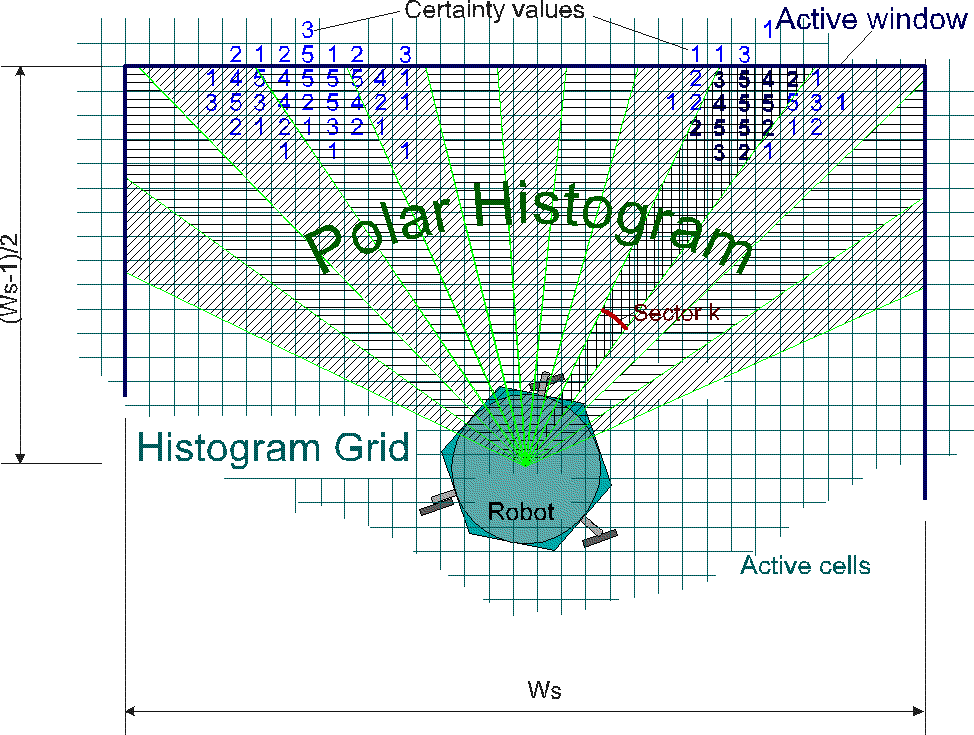
\includegraphics[width=1\textwidth]{vfh_C}
        \caption{Mapping active cells into sectors of the Polar Histogram $H$.}
     \end{figure}
\end{column}\end{columns}
\end{frame}
\begin{frame}{The Vector Field Histogram}{Stage 2/2 of data reduction}
\only<1>{
    \begin{figure}\centering
        \begin{subfigure}{0.5\textwidth}
        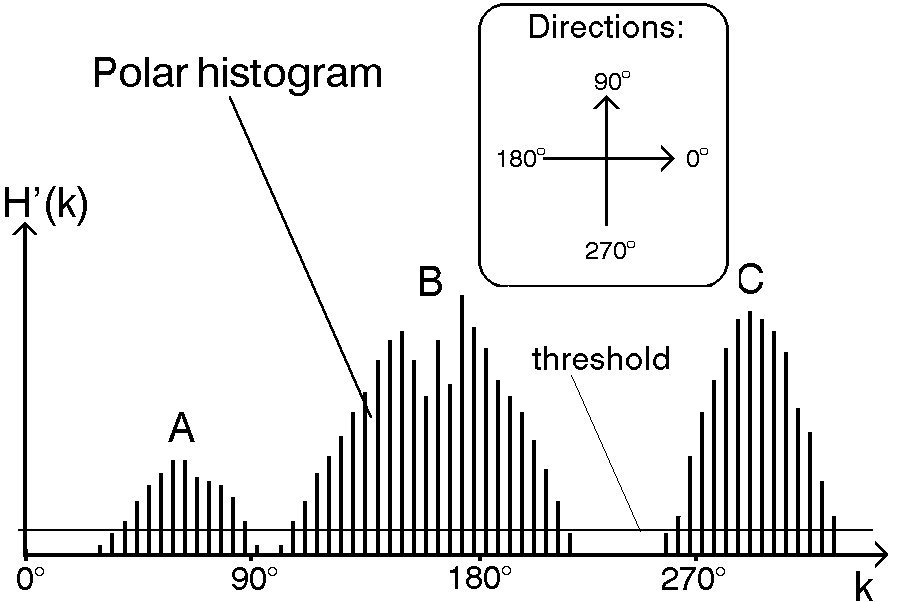
\includegraphics[width=1\textwidth]{vfh_H}
        \caption{1D polar histogram of obstacle occupancy around the robot.}
        \end{subfigure}
        \begin{subfigure}{0.4\textwidth}
        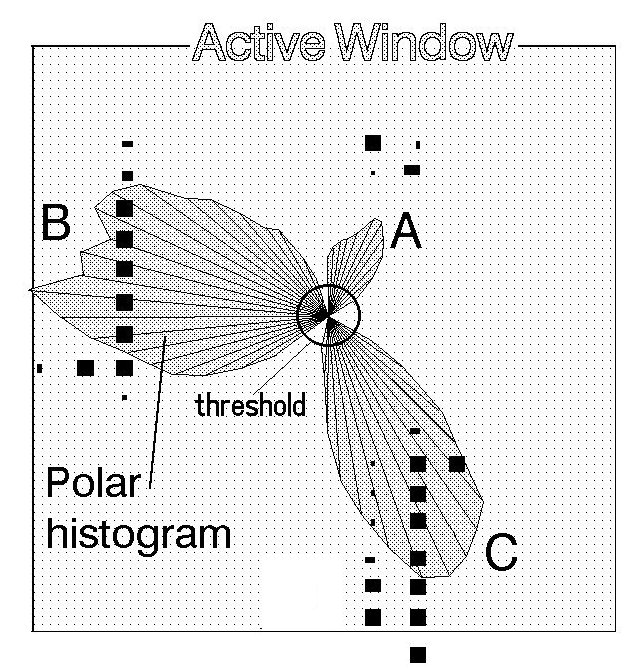
\includegraphics[width=1\textwidth]{vfh_H_C}
        \caption{Polar histogram shown in polar form overlapped with $C^*$.}
        \end{subfigure}
     \end{figure}
}
\only<2>{\begin{columns}
\begin{column}{0.6\textwidth}
\begin{itemize}\small
\item From the set of wide valleys, VHF chooses the one that minimizes a cost function that accounts for:
    \subitem The alignment of the robot to the target,
    \subitem The difference between the robot current direction and the goal direction,
    \subitem The difference between the robot previously selected direction and the new robot direction.
\end{itemize}
\end{column}
\begin{column}{0.4\textwidth}
\begin{figure}\centering
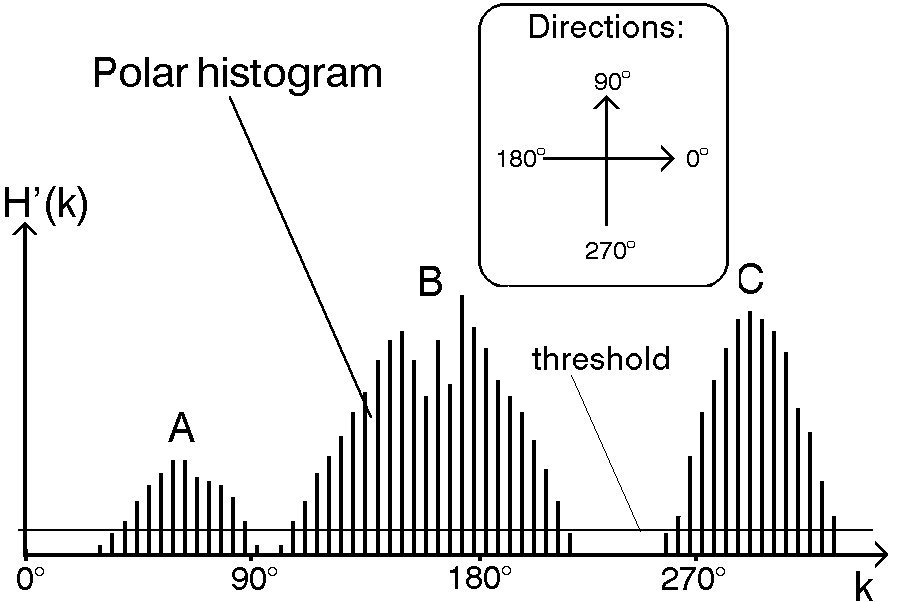
\includegraphics[width=1\textwidth]{vfh_H}
\caption{1D polar histogram of obstacle occupancy around the robot.}
\end{figure}
\end{column}\end{columns}
}
\end{frame}
\begin{frame}{The Vector Field Histogram}{Pros and Cons}
\begin{itemize}
\item The Vector Field Histogram overcomes some of the limitations exhibited by the potential field methods.
    \subitem The influence of bad sensor measurements is minimized because sensorial data is averaged out onto an histogram grid that is further processed.
    \subitem Instability in travelling down a corridor, present when using the potential field method, is eliminated.
    \subitem In the VFH there is no repulsive nor attractive forces and thus the robot cannot be trapped in a local minima.
\end{itemize}
\end{frame}
\section{Conclusion}
\begin{frame}{Conclusion}
\begin{itemize}
\item In this presentation we have reviewed the following obstacle avoidance algorithms:
    \subitem Bug Algorithms
    \subitem The Potential Field Methods
    \subitem The Virtual Force Field
    \subitem The Vector Field Histogram
\end{itemize}
\end{frame}
\section{}
\begin{frame}
    \begin{center}
    \vspace{5em}
    {\fontsize{20}{50}\selectfont Thank You!}
    \end{center}
\end{frame}

\section{References}
\begin{frame}{References}
    \nocite{*}
    {\scriptsize
    \bibliographystyle{IEEEtran}
    \bibliography{reference}
    }
\end{frame}

\appendix

\end{document}